\chapter{}

\section{}
In dieser Aufgabe ist das in der Aufgabe 3 erstellte Subsystem im entsprechenden Block der U/f-Steuerung einzusetzen und deren Implementierung zu testen.\\
Die Ausgangsfrequenz des Umrichters haben wir dabei in 10 Hz-Schritten von 0 Hz bis 100 Hz eingestellt. Die Werte der Ausgangsspannung konnten wir auf Bedienoberfläche ablesen. Wir haben sie mit der Ausgangsfrequenz in eine Tabelle eingetragen und in einem Diagramm dargestellt (Abbildung \ref{fig:6b:UL}). Um die Ausgangsspannung als Effektivwert der Außenleiterspannung darzustellen, haben wir sie nach der (\ref{eq:6:u}) umgerechnet.
\begin{equation}
	U = U_{a}\frac{\sqrt{3}}{\sqrt{2}}
	\label{eq:6:u}
\end{equation}
\begin{figure}[h]
	\centering
	% This file was created by matlab2tikz.
%
%The latest updates can be retrieved from
%  http://www.mathworks.com/matlabcentral/fileexchange/22022-matlab2tikz-matlab2tikz
%where you can also make suggestions and rate matlab2tikz.
%
\definecolor{mycolor1}{rgb}{0.00000,0.44700,0.74100}%
%
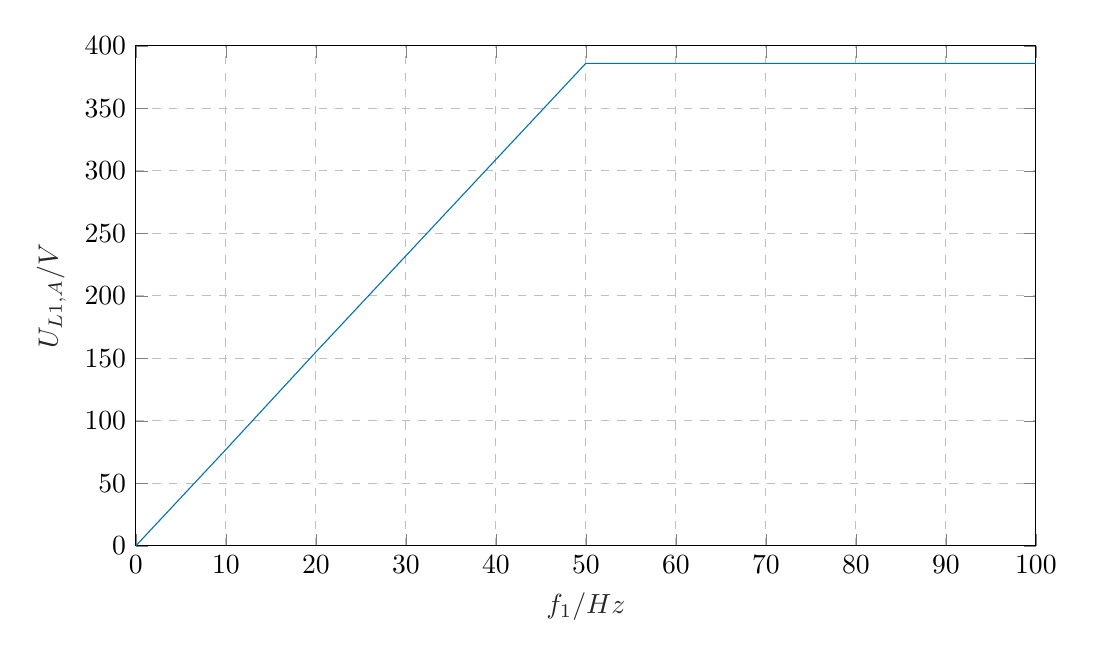
\begin{tikzpicture}

\begin{axis}[%
width=4.5in,
height=2.5in,
at={(0.758in,0.481in)},
scale only axis,
xmin=0,
xmax=100,
xtick={  0,  10,  20,  30,  40,  50,  60,  70,  80,  90, 100},
xlabel style={font=\color{white!15!black}},
xlabel={$ f_{1}/Hz $},
ymin=0,
ymax=400,
ytick={  0,  50, 100, 150, 200, 250, 300, 350, 400},
ylabel style={font=\color{white!15!black}},
ylabel={$ U_{L1,A}/V $},
axis background/.style={fill=white},
xmajorgrids,
ymajorgrids,
major grid style={dashed}
]
\addplot [color=mycolor1, forget plot]
  table[row sep=crcr]{%
0	0\\
10	77\\
20	155\\
30	232\\
40	309\\
50	386\\
60	386\\
70	386\\
80	386\\
90	386\\
100	386\\
};
\end{axis}
\end{tikzpicture}%
	\caption{Gemessene Außenleiterspannung $ U_{L1,A}  $ über Statorfrequenz $ f_{1} $}
	\label{fig:6b:UL}
\end{figure}



\section{}
Im zweiten Aufgabenteil soll der prinzipiellen Verlauf des Betrags der Statorflussverkettung $ \psi_{1} $ und des Kippmoments $ M_{K} $ im Bereich f1 2 [0 100 Hz] dargestellt werden.\\
Die dabei verwendeten Motorparameter sind:
\begin{center}
	$ L_{\mu} = 785.5mH $ \hspace{2cm} $ L_{\sigma} = 209.8mH $
\end{center}
Die Statorflussverkettung $ \psi_{1} $ haben wir mit der Gleichung (\ref{eq:6:psi}) berechnet.
\begin{equation}
	\psi_{1} = \frac{U_{1}}{\Omega_{1}}
	\label{eq:6:psi}
\end{equation}
Der Verlauf des Betrags der Statorflussverkettung $ \psi_{1} $ ist in der Abbildung \ref{fig:6b:psi} dargestellt. Der Verlauf des Kippmoments $ M_{K} $ wird in der Abbildung \ref{fig:6c:Momente} dargestellt.
\begin{figure}[h]
	\centering
	% This file was created by matlab2tikz.
%
%The latest updates can be retrieved from
%  http://www.mathworks.com/matlabcentral/fileexchange/22022-matlab2tikz-matlab2tikz
%where you can also make suggestions and rate matlab2tikz.
%
\definecolor{mycolor1}{rgb}{0.00000,0.44700,0.74100}%
%
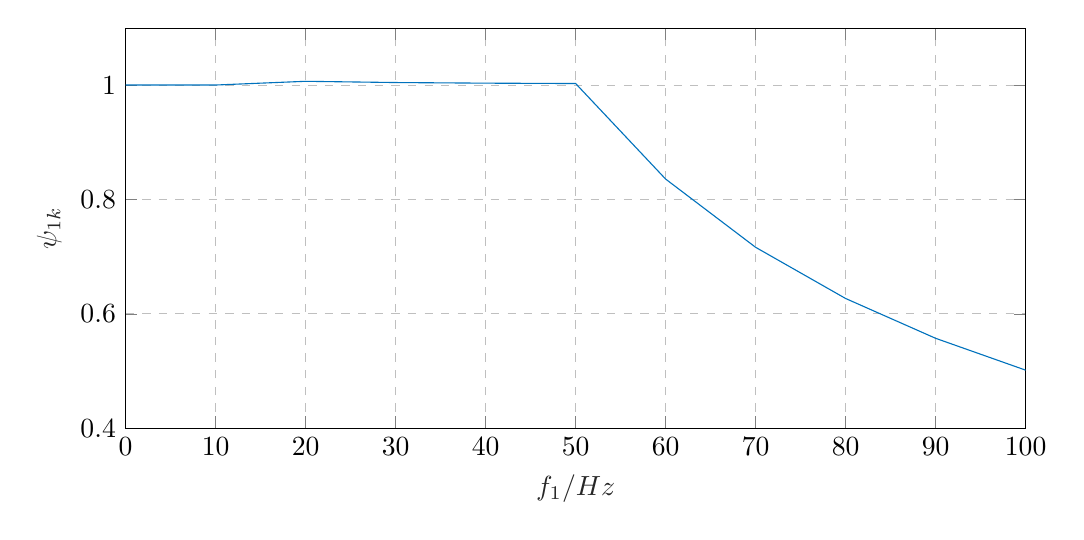
\begin{tikzpicture}

\begin{axis}[%
width=4.5in,
height=2in,
at={(0.758in,0.481in)},
scale only axis,
xmin=0,
xmax=100,
xtick={  0,  10,  20,  30,  40,  50,  60,  70,  80,  90, 100},
xlabel style={font=\color{white!15!black}},
xlabel={$ f_{1}/Hz $},
ymin=0.4,
ymax=1.1,
ylabel style={font=\color{white!15!black}},
ylabel={$ \psi_{1k} $},
axis background/.style={fill=white},
xmajorgrids,
ymajorgrids,
major grid style={dashed}
]
\addplot [color=mycolor1, forget plot]
  table[row sep=crcr]{%
0	1.000610895\\
10	1.000610895\\
20	1.007108368\\
30	1.004942544\\
40	1.003859632\\
50	1.003209884\\
60	0.836008237\\
70	0.716578489\\
80	0.627006178\\
90	0.557338825\\
100	0.501604942\\
};
\end{axis}
\end{tikzpicture}%
	\caption{Statorflussverkettung $ \psi_{1} $ über Statorfrequenz $ f_{1} $}
	\label{fig:6b:psi}
\end{figure}



\section{}
Im letzten Aufgabenteil soll nun der Verlauf des Drehmoments $ M_{Mi}(I_{1N}) $ des Motors zum Verlauf des Kippmoments $ M_{K} $ eingezeichnet werden.\\
Das Drehmoment $ M_{Mi}(I_{1N}) $ wurde mit (\ref{eq:6b:mmi}) berechnet. Es wurde dabei angenommen, dass der Motor bei $ cos\varphi = 0.7 $ betrieben wird. 
\begin{equation}
	M_{Mi} = \frac{3}{2}Z_{P}\frac{U_{1k}}{\Omega_{1}}I_{1N}cos\varphi
	\label{eq:6b:mmi}
\end{equation}
\begin{figure}[h]
	\centering
	% This file was created by matlab2tikz.
%
%The latest updates can be retrieved from
%  http://www.mathworks.com/matlabcentral/fileexchange/22022-matlab2tikz-matlab2tikz
%where you can also make suggestions and rate matlab2tikz.
%
\definecolor{mycolor1}{rgb}{0.00000,0.44700,0.74100}%
\definecolor{mycolor2}{rgb}{0.85000,0.32500,0.09800}%
%
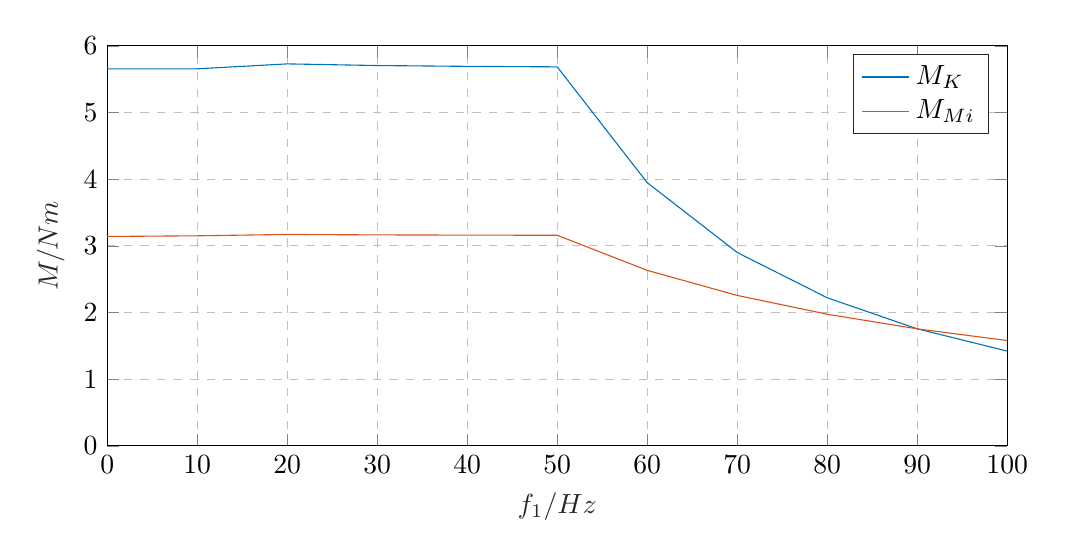
\begin{tikzpicture}

\begin{axis}[%
width=4.5in,
height=2in,
at={(0.758in,0.481in)},
scale only axis,
xmin=0,
xmax=100,
xtick={  0,  10,  20,  30,  40,  50,  60,  70,  80,  90, 100},
xlabel style={font=\color{white!15!black}},
xlabel={$ f_{1}/Hz $},
ymin=0,
ymax=6,
ytick={0, 1, 2, 3, 4, 5, 6},
ylabel style={font=\color{white!15!black}},
ylabel={$ M/Nm $},
axis background/.style={fill=white},
xmajorgrids,
ymajorgrids,
legend style={legend cell align=left, align=left, draw=white!15!black},
major grid style={dashed}
]
\addplot [color=mycolor1]
  table[row sep=crcr]{%
0	5.655088301\\
10	5.655088301\\
20	5.728769457\\
30	5.704156083\\
40	5.691869266\\
50	5.684503535\\
60	3.947571899\\
70	2.900256906\\
80	2.220509193\\
90	1.7544764\\
100	1.421125884\\
};
\addlegendentry{$ M_{K} $}

\addplot [color=mycolor2]
  table[row sep=crcr]{%
0	3.14\\
10	3.149962511\\
20	3.170416813\\
30	3.163598712\\
40	3.160189662\\
50	3.158144232\\
60	2.63178686\\
70	2.255817309\\
80	1.973840145\\
90	1.754524573\\
100	1.579072116\\
};
\addlegendentry{$ M_{Mi} $}

\end{axis}
\end{tikzpicture}%
	\caption{Kippmoment $ M_{K} $ und inneres Moment $ M_{Mi} $ über Statorfrequenz $ f_{1} $}
	\label{fig:6c:Momente}
\end{figure}